We apply a data-driven method to correct for instrumental effects on the jet 
counting efficiencies and its associated systematic uncertainties. 
In this method, the $H \to \ZZ$ jet counting efficiency in data 
$\epsilon_{H \to \ZZ}$ is corrected by a data-to-simulation scale factor 
obtained by comparing the jet counting efficiency in $\dyll$ enriched 
events in data with the value from simulation, 

$$\epsilon_{H \to \ZZ} = \epsilon_{\Z}^{data} (\frac{\epsilon_{H \to \ZZ}}{\epsilon_{\Z}})^{MC}.$$

The observed data-to-simulation correction factors are 
close to unity for the zero-jet and 1-jet bins.
% while we observe some disagreement for events with at least two reconstructd jets. 
%This is not surprising since Powheg is an NLO generator, and 
%only expected to produce an accurate description for events 
%containing up to one jet. For instance, the comparison between data and Madgraph 
%simulation, which accounts for leading order diagrams containing up to four additional
%partons, gives much better agreement in the 2-jet bin. 
As a result no correction is applied on top of the jet spectrum simualated 
for the Higgs signal, reweighted the Higgs $\pt$ spectrum is to the NNLO+NNLL differential calculation. 
%The jet multiplicity distribution for $\dyll$ events is shown in 
%Figure~\ref{fig:njets_dyll}. Events with at least two reconstructed jets have been 
%reweighted by a factor 1.6, which is the observed ratio between Madgraph and 
%Powheg simulated events.

%\begin{figure}[!htbp]
%\begin{center}
%   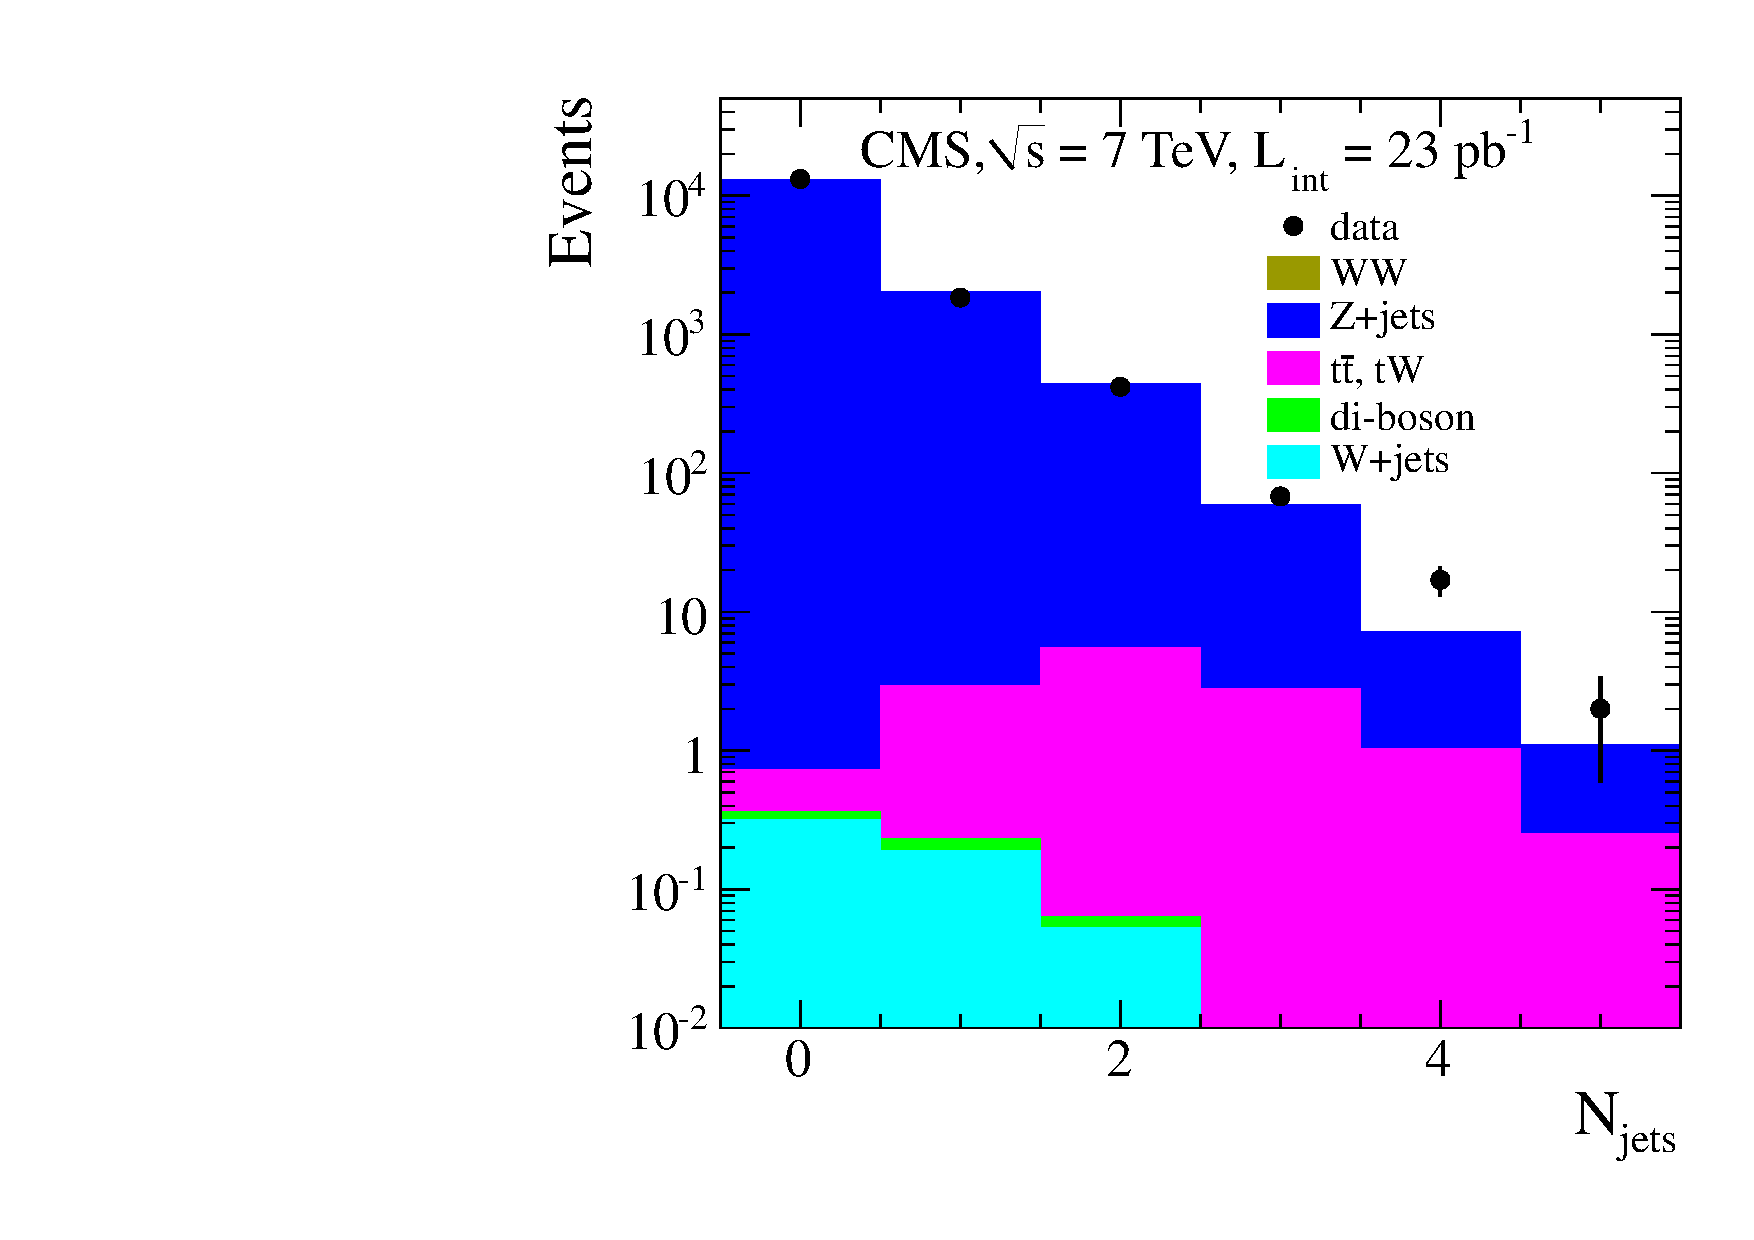
\includegraphics[width=0.60\textwidth]{figures/njets_dyll.pdf}
%   \caption{Jet multiplicity distribution for $\dyll$ events.}
%   \label{fig:njets_dyll}
%\end{center}
%\end{figure}
